\section{Aufgabe: Kragarm (2D)}
\begin{figure}[!ht]
\centering
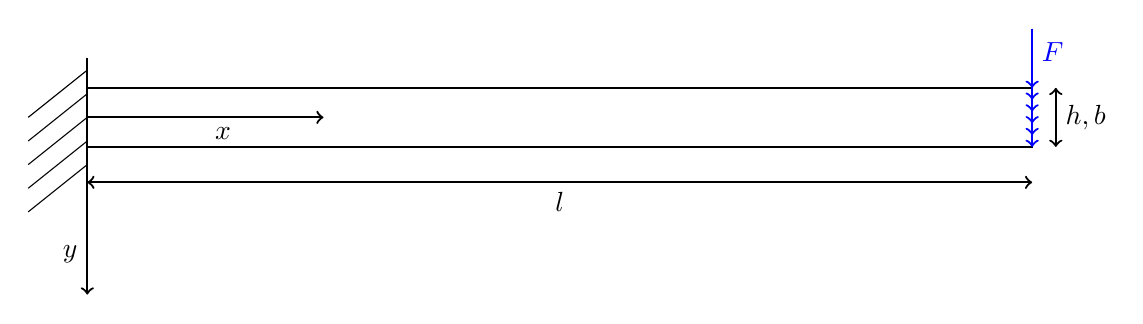
\begin{tikzpicture}[scale=1.5]
    % Beam
    \draw[thick] (0,0) rectangle (8,0.5);
    % Fixed support (left side)
    \draw[thick] (0,0.75) -- (0,-0.25);
    % Schraffuren (parallele Linien für die Auflagerung)
    \draw[] (-0.5,0.25) -- (0,0.65);
    \draw[] (-0.5,0.05) -- (0,0.45);
    \draw[] (-0.5,-0.15) -- (0,0.25);
    \draw[] (-0.5,-0.35) -- (0,0.05);
    \draw[] (-0.5,-0.55) -- (0,-0.15);
    % Force arrow
    \draw[->, thick, blue] (8,1) -- (8,0.5);
    \draw[->, thick, blue] (8,1) -- (8,0.4);
    \draw[->, thick, blue] (8,1) -- (8,0.3);
    \draw[->, thick, blue] (8,1) -- (8,0.2);
    \draw[->, thick, blue] (8,1) -- (8,0.1);
    \draw[->, thick, blue] (8,1) -- (8,0.0);
    \node[blue, right] at (8,0.8) {$F$};
    % Labels
    % \node[below] at (4,0) {Balken};
    
    % Koordinatensystem am Ursprung (0,0)
    % x-Achse (horizontal nach rechts)
    \draw[->, thick, black] (0,0.25) -- (2,0.25);
    \node[below right] at (1,0.25) {$x$};
    % z-Achse (vertikal nach unten)
    \draw[->, thick, black] (0,0.25) -- (0,-1.25);
    \node[below left] at (0,-0.75) {$y$};
    
    % Länge l (unten unter dem Balken)
    \draw[<->, thick] (0,-0.3) -- (8,-0.3);
    \node[below] at (4,-0.3) {$l$};
    
    % Höhe h (vertikal am rechten Ende des Balkens)
    \draw[<->, thick] (8.2,0) -- (8.2,0.5);
    \node[right] at (8.2,0.25) {$h, b$};
\end{tikzpicture}
\caption{Schematische Darstellung des Kragarms mit Einspannung, Koordinatensystem, Länge $l$, Höhe $h$ und Auflast $F$}
\label{fig:kragarm-schematik}
\end{figure}

Als Balken wird ein quadratisches Profil verwendet. Die materialspezifischen Parameter wie der Elastizitätsmodul \cite[S. 43]{gomeringer_tabellenbuch_2024} $E$ und die Poissonzahl \cite[S. 67]{gross_technische_2021} $\nu$ werden für einen unlegierten Stahl gewählt.
Es werden folgende Parameter gewählt :

\begin{table}[h]
\centering
\caption{Ausgewählte Parameter für den Kragarm}
\label{tab:parameter}
\begin{tabular}{ll}
\toprule
Parameter & Wert \\
\midrule
Elastizitätsmodul $E$ & \num{210000} \si{\pascal} \\
Poisson-Zahl $\nu$ & \num{0.3} \\
Länge $l$ & \num{2} \si{\meter} \\
Kraft $F$ & \num{1000} \si{\newton} \\
Höhe $h$ & \num{0.05} \si{\meter} \\
Breite $b$ & \num{0.05} \si{\meter} \\
\bottomrule
\end{tabular}
\end{table}

\subsection{Berechnung des Balkens nach Bernoulli}
\label{Bernoulli}
Es sollen die maximale Biegespannung $\sigma_\text{max}$, die maximale Verzerrung $\epsilon_\text{max}$ und die maximale Durchbiegung $w_\text{max}$ bestimmt werden.
Das maximale Biegemoment beträgt

\begin{equation}
M_\text{max} = F \cdot l = \SI{1000}{\newton} \cdot \SI{2}{\meter} = \SI{2000}{\newton\meter}
\end{equation}

Das Flächenträgheitsmoment $I$ für einen rechteckigen Querschnitt ist

\begin{equation}
I_z = \frac{b \cdot h^3}{12} = \frac{b^4}{12} = \frac{(\SI{0.05}{\meter})^4}{12} = \SI{5.208333e-7}{\meter\tothe{4}}
\end{equation}

Die maximale Biegespannung $\sigma$ ergibt sich aus
\begin{equation}
\sigma_\text{max} = \frac{M_\text{max} \cdot (h/2)}{I} = \SI{960e5}{\pascal} = \SI{96}{\mega\pascal}
\end{equation}

Die maximale Verzerrung / Dehnung $\epsilon$  folgt aus dem Hookeschen Gesetz

\begin{equation}
\epsilon_\text{max} = \frac{\sigma_\text{max}}{E} = \SI{4,57e-4}{}
\end{equation}

Aus der Biegeliniendifferentialgleichung folgt die maximale durchsenkung $w_\text{max}$:

\begin{equation}
w_\text{max} = \frac{F \cdot L^3}{3 \cdot E \cdot I} = \SI{2,438e-2}{\meter} = \SI{24,38}{\milli\meter}
\end{equation}

\subsection{Berechnung mit 2D-FEM-Solver - Python}

Das Programm löst eine lineare, eben gespannte 2D-FE-Aufgabe (Ebener Spannungszustand) eines Kragarms (Balken) mit bilinearen Viereckselementen (Q4) in PyTorch. Randbedingungen: Einspannung am linken Rand, Linienlast (Querkraft) am rechten Rand. Neben Verschiebungen werden Spannungen, Dehnungen und Vergleichsspannungen berechnet und grafisch dargestellt. Die analytische Biegelösung durch Bernoulli-Balkentheorie dient der Verifikation.


\subsubsection{Versuchsaufbau - Packages \& Versionen}
Die numerische Untersuchung des dargestellten Problems basiert auf einer eigens entwickelten Finite-Elemente-Implementierung in der Programmiersprache \texttt{Python}. %Diese Wahl begründet sich in der hohen Abstraktionsfähigkeit der Sprache sowie dem Zugriff auf ein maturisiertes Ökosystem an Bibliotheken für wissenschaftliches Rechnen, welches eine schnelle und verifizierbare Prototypentwicklung ermöglicht.
Das Kernstück der numerischen Analyse bildet das Framework \texttt{PyTorch}. Primär für Applikationen des maschinellen Lernens konzipiert, stellt es eine hochoptimierte Umgebung für Tensor-basierte Berechnungen zur Verfügung, deren Eigenschaften sich als vorteilhaft für die Implementierung der Finite-Elemente-Methode erweisen:
\begin{itemize}
\item \textbf{Tensor-Algebra:} Sämtliche relevanten physikalischen und mathematischen Entitäten – wie Koordinatenvektoren, der Verschiebungsvektor \textit{u} oder die globale Steifigkeitsmatrix \textit{K} – werden als mehrdimensionale Tensoren abgebildet. Dies ermöglicht eine syntaktisch prägnante und mathematisch intuitive Formulierung der FEM-Algorithmen.
\item \textbf{Rechenleistung:} Die Fähigkeit zur transparenten Parallelisierung von Berechnungen auf modernen Multi-Core-Prozessoren wurde in der vorliegenden Implementierung genutzt, um die Recheneffizienz zu steigern. Darüber hinaus bietet \texttt{PyTorch} die Möglichkeit zur nahtlosen Ausführung auf Grafikprozessoren (GPUs), was bei größeren Modellen eine signifikante Reduktion der Rechenzeit ermöglicht.
\item \textbf{Numerische Präzision:} Um die Akkumulation von Rundungsfehlern zu minimieren und eine hohe Genauigkeit der Ergebnisse sicherzustellen, wurde der standardmäßige Datentyp für alle Fließkommaoperationen auf 64-Bit (\texttt{torch.float64}) festgelegt.
\end{itemize}
Zur Datenverarbeitung und insbesondere zur Visualisierung der Ergebnisse kamen die etablierten Bibliotheken \texttt{NumPy} und \texttt{Matplotlib} zum Einsatz. \texttt{NumPy} stellt die fundamentalen Datenstrukturen für numerische Operationen bereit und sichert die Interoperabilität im wissenschaftlichen Python-Ökosystem. \texttt{Matplotlib} diente als primäres Werkzeug für die grafische Aufbereitung aller Simulationsergebnisse, von der Darstellung des diskretisierten Modells bis hin zur Visualisierung der Spannungsfelder und dem Vergleich mit der analytischen Lösung.
Diese sorgfältig ausgewählte Kombination von Software-Komponenten bildet eine robuste und leistungsfähige Basis für die Durchführung und Analyse der numerischen Simulationen im Rahmen dieser Arbeit.






\subsubsection{Modellaufbau}

\label{sec:modellaufbau}

\paragraph{Grundlegende Annahmen: \ac{ESZ}}\\
Das FEM-Modell basiert auf der Annahme eines \textbf{Ebenen Spannungszustandes (ESZ)}. Diese Annahme ist gültig für dünne Strukturen, bei denen die Dicke (hier \texttt{width = 0.05}\,m) klein im Vergleich zur Länge und Höhe ist.

\begin{itemize}
    \item Im ESZ wird angenommen, dass Spannungen normal zur Ebene (z-Richtung) null sind: $\sigma_{zz} = \sigma_{xz} = \sigma_{yz} = 0$.
    \item \textbf{Korrektur zur Annahme $\sigma_{yy} = 0$:} Die Annahme $\sigma_{yy} = 0$ (wie in der 1D-Balkentheorie) wird hier \emph{nicht} getroffen. Im 2D-ESZ-Modell wird $\sigma_{yy}$ (Pressung/Zug in y-Richtung) infolge der Querkontraktion ($\nu = 0.3$) korrekt berechnet. Dies wird im Code durch die vollständige ESZ-Materialmatrix \texttt{C4} sichergestellt.
\end{itemize}

\paragraph{Diskretisierung: Netz und Elementtyp}

\subparagraph{Elementtyp: Planes 4-Knotenelement (Q4)}
Das 2D-Gebiet (Balken) wird mit \textbf{ebenen 4-Knotenelementen} (im Code \texttt{nen = 4}) diskretisiert.

\begin{itemize}
    \item \textbf{Freiheitsgrade:} Jeder der vier Knoten besitzt zwei translatorische Freiheitsgrade (DOFs): Verschiebung in x-Richtung ($u_x$) und Verschiebung in y-Richtung ($u_y$). Ein Element hat somit 8 DOFs.
    \item \textbf{Ansatzfunktionen:} Die Verschiebung innerhalb des Elements wird über \textbf{bilineare Ansatzfunktionen} (z.B. $N_1 = 0.25 (1-\xi)(1-\eta)$) interpoliert. Diese sind, wie gefordert, \emph{linear} in den lokalen $\xi$- und $\eta$-Koordinaten, nicht quadratisch.
\end{itemize}

\subparagraph{Netzaufbau (Elemente und Knoten)}
Die Diskretisierung erfolgt durch ein strukturiertes Gitter, das prozedural erzeugt wird:

\begin{itemize}
    \item \textbf{Geometrie:} Balkenlänge \texttt{length = 2.0}\,m, Höhe \texttt{height = 0.05}\,m.
    \item \textbf{Elementform:} Das Netz wird mit \texttt{nx = 120} Elementen in Längsrichtung und \texttt{ny = 10} Elementen in Höhenrichtung erstellt. Dies erzeugt \textbf{rechteckige Elemente} (Elementabmessungen $\Delta x \approx 0.0167$\,m und $\Delta y = 0.005$\,m), die unverzerrt sind, was numerisch vorteilhaft ist.
    \item \textbf{Element-Knoten-Vergleich:} Das Modell besteht aus:
        \begin{itemize}
            \item \texttt{nel = nx * ny = 120 * 10 =} \textbf{1200 Elementen}
            \item \texttt{nnp = (nx + 1) * (ny + 1) = 121 * 11 =} \textbf{1331 Knoten}
        \end{itemize}
\end{itemize}

\subparagraph{Integration}
Die Elementsteifigkeitsmatrizen werden numerisch integriert. Es wird eine \textbf{volle Integration} mittels \textbf{2x2-Punkt-Gauß-Quadratur} verwendet (\texttt{nqp = 4}). Dies ist die exakte Integrationsordnung für bilineare Q4-Elemente bei rechteckiger Geometrie und verhindert "Hourglassing" bei geringer schiefe der Elemente.

\paragraph{Randbedingungen und Lasten}

Der Rand des betrachteten Gebietes stellt mathematisch den Rand des Definitionsbereichs unseres Differentialgleichungssystem. Für dieses Randwertprobem sind entweder Dirichlet-Randbedingungen (bei denen die Funktionswerte - hier Verschiebungen - auf dem Rand vorgegeben sind) oder Neumann-Randbedingungen (bei denen die Ableitungswerte - hier Last - vorgegeben sind).

muss per Definition eine Randbedingung besitzen, dabei 

\subparagraph{Dirichlet-Randbedingung (Lagerung)}
Am linken Ende des Balkens ($x=0$) wird eine Einspannung realisiert.

\begin{itemize}
    \item \textbf{Bedingung:} Alle Knoten (\texttt{left\_nodes}) an dieser Kante werden in ihren Verschiebungen blockiert ($u_x = 0$ und $u_y = 0$).
    \item \textbf{Implementierung (Penalty-Methode):} Die Dirichlet-Ranbedingungen werden über die \textbf{Penalty-Methode} implementiert. Anstatt das Gleichungssystem zu reduzieren, wird die globale Steifigkeitsmatrix \texttt{K} modifiziert: Auf die Diagonaleinträge der Freiheitsgrade, die festgehalten werden sollen, wird ein sehr großer Steifigkeitswert (im Code \texttt{1e22}) addiert. Diese "Strafterme" in der \texttt{drlt\_matrix} erzwingen numerisch, dass die Verschiebungen an diesen Stellen (nahezu) null werden, um die Systemgleichung $K \cdot u = F$ zu erfüllen.
\end{itemize}

\subparagraph{Neumann-Randbedingungen (Kräfte)}
Alle anderen Ränder des Gebiets sind Neumann-Ränder.

\begin{itemize}
    \item \textbf{Freie Ränder (Balkenlänge):} An der Ober- und Unterseite des Balkens gilt die Bedingung $t=0$ (Traktionsvektor/Spannungsvektor ist null). Dies ist die "natürliche" Randbedingung in der FEM und muss nicht explizit implementiert werden; es werden einfach keine Kräfte auf diese Knoten aufgebracht.
    \item \textbf{Lastaufbringung (Endfläche):} Am rechten Ende ($x=L$) wird eine Gesamtkraft \texttt{F = 1000.0}\,N als \textbf{Linienlast} aufgebracht (\texttt{total\_force = -F / width}). Diese Kraft wird im Code gleichmäßig auf alle Knoten am rechten Rand (\texttt{right\_nodes}) aufgeteilt und als diskrete Knotenkräfte \texttt{force\_per\_node} in negativer y-Richtung in den globalen Lastvektor eingetragen.
\end{itemize}


\subsubsection{Programmstruktur und Ablauf}

Die Prozedur in \texttt{FEM2\_HA1\_Diskretisierer} ist vollständig in der Funktion \texttt{analysis()} implementiert. 
Der Ablauf gliedert sich in Konfiguration, Netzaufbau, Materialdefinition, Lösung und Post-Processing:

\begin{itemize}
  \item \textbf{Globale Einstellungen}: Datentyp und Threads (\texttt{torch.set\_default\_dtype(float64)}, \texttt{set\_num\_threads(4)}), Plot-Flags (\texttt{toplot}, \texttt{disp\_scaling}), sowie Material-, Geometrie- und Diskretisierungsparameter (\(E, \nu, L, H, b, NX\\, NY, NEN = 4, nqp = 4\)).
  
  \item \textbf{Geometrie und Randbedingungen}: Reguläres Q4-Gitter (\(\mathbf{x}, \mathbf{T}\)); Einspannung bei \(x=0\), gleichmäßig verteilte Linienlast in y-Richtung bei \(x=L\).
  
  \item \textbf{Materialmodell}: Isotrop linear-elastisch (plane stress) mit Materialmatrix \(\mathbf{C}(E, \nu)\) und Schubmodul 
  \[
  G = \frac{E}{2(1+\nu)}.
  \]
  
  \item \textbf{Numerik}: 2×2-Gaußquadratur, Gestaltfunktionen \(N\) und \(\partial N / \partial \xi\), Freiheitsgrad- und Randmasken (\texttt{edof}, \texttt{gdof}, \texttt{drlt\_mask}, \texttt{neum\_vals}), sowie Penalty-Matrix
  \[
  \mathbf{K}^{\text{pen}} = 10^{22} \, \mathrm{diag}(\texttt{drlt\_mask}).
  \]
  
  \item \textbf{Solver}: Assemblierung von \(\mathbf{K}\) und \(\mathbf{f}^{\text{int}}\); Lösung des linearen Gleichungssystems
  \[
  (\mathbf{K} + \mathbf{K}^{\text{pen}})\mathbf{u} = \mathbf{f}^{\text{neu}} - \mathbf{f}^{\text{int}}
  \]
  mit \texttt{torch.linalg.solve}.
  
  \item \textbf{Post-Processing}: Berechnung und Visualisierung von Spannungen (\(\sigma_{xx}, \sigma_{yy}, \sigma_{\text{vM}}\)), Verschiebungen (\(u_x, u_y\)) und Dehnungen (\(\varepsilon_{xx}\)); Vergleich mit der analytischen Biegetheorie bei \(x = L/2\).
\end{itemize}

\subsubsection{Numerischer Ablauf im Element}

Für jedes Element \(e\) und jeden Gaußpunkt \(q\) erfolgt die Berechnung gemäß:
\[
\mathbf{J} = \mathbf{x}_e \boldsymbol{\Gamma}, \qquad
\mathbf{G} = \boldsymbol{\Gamma} \mathbf{J}^{-1},
\]
\[
\boldsymbol{\varepsilon} = \tfrac{1}{2} \left( \mathbf{u}_e \mathbf{G} + (\mathbf{u}_e \mathbf{G})^\top \right), \qquad
\boldsymbol{\sigma} = \mathbf{C} : \boldsymbol{\varepsilon}.
\]
Die Beiträge zur inneren Kraft und zur Steifigkeitsmatrix ergeben sich zu:
\[
\mathbf{f}^{\text{int}}_A \;{+}{=}\; \sum_q w_q \, \det(\mathbf{J}) \, \mathbf{G}_A \, \boldsymbol{\sigma}, \qquad
\mathbf{K}_{AB} \;{+}{=}\; \sum_q w_q \, \det(\mathbf{J}) \, (\mathbf{G}_A : \mathbf{C} : \mathbf{G}_B).
\]

Global wird schließlich gelöst:
\[
(\mathbf{K} + \mathbf{K}^{\text{pen}})\mathbf{u} = \mathbf{f}^{\text{neu}} - \mathbf{f}^{\text{int}}.
\]

\subsubsection{Konfiguration und Reproduzierbarkeit}

 Alle relevanten Parameter (\(E, \nu, L, H, b, NX, NY, \texttt{FORCE}\)) sowie numerische Einstellungen (\texttt{float64}, \texttt{torch.set\_n\\um\_threads(4)}) und Plotoptionen werden zentral in \texttt{analysis()} definiert, sodass das Skript vollständig reproduzierbar bleibt.




\subsection{Berechnung mit 2D-FEM-Solver - Ansys Mechanical}
Um den 2D-FEM-Solver aus Python bestmöglich zu validieren, wurde ein 2D-Modell innerhalb einer komerziell etablierten Software-Suite erstellt und berrechnet.


\subsubsection{Versuchsaufbau}
Das Modell wurde innerhalb Ansys Mechanical 2025R2 Student Edition \cite{noauthor_download_nodate} aufgebaut und berechnet. Dabei unterstützt das Programm durch eine komplett in GUI's integrierte Benutzerführung, die sowohl das Präprozessing, Prozessing, als auch das Postprozessing ermöglicht.

Durch die Benutzung der \ac{FEM}-Software hat man die Möglichkeit über einfache Einstellmasken das Modell aufzubauen, wobei die genauen Lösungsbedingungen des Problems und die verwendeten Elementformulierungen über tiefergehende Untersuchungen herauszufinden sind.

\subsection{Modellaufbau}
Es wurde eine Fläche mit den identischen Abmaßen wie in \cref{tab:parameter} festgelegt erstellt.
Diese Fläche wurde in Ansys Mechanical diskretisiert und den identischen Randbedingungen wie auch bei der analytischen Lösung ausgesetzt.

\begin{figure}[ht]
    \centering
    \includegraphics[width=0.75\linewidth]{Bilder/2D Balken unvernetzt.png}
    \caption{Balken als 2D Fläche}
    \label{fig:Balken als 2D Fläche}
\end{figure}

Für diesen 2D Balken wird ein ebener Spannungszustand angenommen.
Es wird eine volle Intergration durchgeführt.

\subsubsection{Elementtyp}

\textbf{PLANE182:} Ein 2D-4-Knoten-Festkörperelement (Quadrilateral) für die Modellierung von 2D-Festkörperstrukturen unter Plane-Stress-, Plane-Strain-, generalisierter Plane-Strain- oder axisymmetrischer Belastung (mit/ohne Torsion). Jeder Knoten hat zwei Freiheitsgrade: UX (Translation in X) und UY (Translation in Y); bei axisymmetrischer Torsion (KEYOPT(3)=6) kommt ROTY hinzu. Die Ansatzfunktionen sind linear.

Ansys: KEYOPT(1) = 2 (enhanced strain formulation).\\

Die Formulierung verwendet eine erweiterte Deformationsansatz mit vier internen (nicht zugänglichen) Freiheitsgraden zur Verbesserung der Schubverzerrungen und Reduzierung von Volumen-Locking bei fast inkompressiblen Materialien. Dies minimiert Locking-Effekte in Biege- und Schubbeanspruchungen im Vergleich zur Standard-Integration (KEYOPT(1)=0). Weitere KEYOPT-Optionen: KEYOPT(3)=0 für Plane Stress, KEYOPT(6)=1 für mixed u-P-Formulierung bei inkompressiblen Elastoplastizitätsmodellen (erfordert Sparse-Solver).


\newpage
\section{Ergebnisse}
In diesem Kapitel werden die Ergebnisse der durchgeführten Berechnungen und Simulationen vorgestellt. Die Darstellung der Resultate gliedert sich entsprechend der drei in dieser Arbeit untersuchten Modellansätze.

Zunächst werden in Abschnitt \ref{subsec:Bernoulli} die Ergebnisse des analytischen bzw. vereinfachten Modells vorgestellt, das auf der Bernoulli-Balkentheorie basiert. 
Darauf folgt in Abschnitt \ref{subsec:ergebnisse_pytorch} die Präsentation der Ergebnisse des selbst implementierten 2D-\ac{FEM}-Modells, welches unter Verwendung von Python und der PyTorch-Bibliothek entwickelt wurde. 
Abschließend werden in Abschnitt \ref{subsec:ergebnisse_ansys} die Resultate der Simulation mit dem kommerziellen FEM-Softwarepaket Ansys dargelegt.

Eine detaillierte vergleichende Analyse und Diskussion dieser drei Ergebnisdatensätze erfolgt im nachfolgenden Kapitel \ref{sec:vergleich}.
Für die Verifizierung der Ergebnisse wird sich einer kommerziellen \ac{FEM}-Software bedient. Wir nutzen Ansys Mechanical.

\subsection{Modell 1: Ergebnisse der Bernoulli-Balkentheorie}
\label{subsec:Bernoulli}
Die Berechnung der Ergenisse für einen Biegebalken wurden bereits in Kapitel \ref{Bernoulli} erledigt und werden deshalb hier nicht erneut erwähnt beziehungsweise aufgeführt.




% \lipsum[1] % Beispieltext
% \begin{figure}[h]
%     \centering
%     % \includegraphics[width=0.8\textwidth]{pfad/zum/bild_bernoulli.png}
%     \caption{Ergebnisdarstellung Bernoulli-Balken.}
%     \label{fig:bernoulli_results}
% \end{figure}


\subsection{Modell 2: Ergebnisse des 2D-FEM Python/PyTorch-Modells}
\label{subsec:ergebnisse_pytorch}

\begin{figure}[!ht]
\centering
\includegraphics[width=0.4\textwidth]{Bilder/Python sigma_xx.png}
\caption{Python Balken - Normalspannung}
\end{figure}

\begin{figure}[!ht]
\centering
\includegraphics[width=0.4\textwidth]{Bilder/Python Verschiebung y-Richtung.png}
\caption{Python Balken - Verschiebung}
\end{figure}

% \lipsum[2] % Beispieltext
% \begin{figure}[h]
%     \centering
%     % \includegraphics[width=0.8\textwidth]{pfad/zum/bild_pytorch.png}
%     \caption{Ergebnisdarstellung 2D-FEM (PyTorch).}
%     \label{fig:pytorch_results}
% \end{figure}


Die hier gezeigten Werte wurden mit einem Netz von 120 Elementen über die Länge und 10 Elementen in der Höhe erreicht.


\newpage

\subsection{Modell 3: Ergebnisse des 2D-FEM Ansys-Modells}
\label{subsec:ergebnisse_ansys}

%Grafik 2D-Modell
\begin{figure}[h]
    \centering
    \includegraphics[width=0.8\linewidth]{Bilder/2D Balken_Verschiebung.png}
    \caption{Diskret. Balken - Verschiebung}
    \label{fig:2D Ansys Modell}
\end{figure}

%Grafik Normalspannung dis. Balken
\begin{figure}[h!]
\centering
\includegraphics[width=0.8\textwidth]{Bilder/2D Balken_max Normalspannung.png}
\caption{Diskret. Balken - Normalspannung}
\label{fig:2D: Python vs Ansys}
\end{figure}

Die hier gezeigten Werte wurden mit einem Netz von 120 Elementen über die Länge und 10 Elementen in der Höhe erreicht.

\newpage

\section{Vergleich der Ergebnisse}
\label{sec:vergleich}

Bei identischer Vernetzung der Modelle mit jeweils:
\begin{itemize}
    \item 10 Elemente entlang der Höhe
    \item 120 Elemente entlang der Länge
\end{itemize}

kommen folgende Ergebnisse zustande:

\begin{table}[h]
    \centering
    \begin{tabular}{|c|c|c|c|}
        \hline
        \textbf{Balkenmodell} & \textbf{Verschiebung in y-Richtung in \si{\milli\meter}} &  \textbf{Normalspannung $\sigma_{xx}$ in \si{\mega\pascal}}\\
        
        \hline
        
        Balkentheorie & 24,38 & 96 \\
        
        \hline
        
        Diskret. Balken Python & 23,35 & 99,4 \\
        \hline
            
        Diskret. Balken Ansys & 23,35 & 99,4 \\
        
        \hline
    \end{tabular}
    \caption{Vergleich der Ergebnisse bei Vernetzung 1}
    \label{tab:Vergleich der Ergebnisse bei Vernetzung 1}
\end{table}


Bei identischer Vernetzung der Modelle mit jeweils:
\begin{itemize}
    \item 8 Elemente entlang der Höhe
    \item 320 Elemente entlang der Länge
\end{itemize}

gehen wir von einer quadratischen Form eines einzelnen Element aus.

\begin{table}[h]
    \centering
    \begin{tabular}{|c|c|c|c|}
        \hline
        \textbf{Balkenmodell} & \textbf{Verschiebung in y-Richtung in \si{\milli\meter}} &  \textbf{Normalspannung $\sigma_{xx}$ in \si{\mega\pascal}}\\
        
        \hline
        
        Balkentheorie & 24,38 & 96 \\
        
        \hline
        
        Diskret. Balken Python & 24,2 & 107,8 \\
        \hline
            
        Diskret. Balken Ansys & 24,2 & 107,83 \\
        
        \hline
    \end{tabular}
    \caption{Vergleich der Ergebnisse bei Vernetzung 2}
    \label{tab:Vergleich der Ergebnisse bei Vernetzung 2}
\end{table}


Wie die Ergebnisse in Tabelle~\ref{tab:Vergleich der Ergebnisse bei Vernetzung 1} zeigen, liefert die Finite-Elemente-Methode
sowohl in der kommerziellen Software \textit{ANSYS} als auch in der eigenen Implementierung mit Python
bei gleicher Diskretisierung eine sehr gute Approximation der analytischen Lösung nach der
Bernoulli-Balkentheorie. 

Für die erste betrachtete Vernetzung (10 Elemente in Höhe, 120 Elemente in Längsrichtung)
beträgt der relative Fehler der maximalen Verschiebung
für den Python-Code etwa \SI{-4.22}{\percent}, ebenso \SI{-4.22}{\percent} für ANSYS.
Die maximale Normalspannung \(\sigma_{xx}\) wird in beiden numerischen Modellen mit \SI{99.4}{MPa}
gegenüber dem Bernoulli-Wert von \SI{96.0}{MPa} um etwa \SI{+3.54}{\percent} überschätzt.

Bei feineren Netzgrößen (10 Elemente in der Höhe, 320 Elemente in der Länge) konvergiert die
Verschiebung deutlich: die numerischen Werte liegen nun bei \SI{24.20}{mm} (Python und ANSYS),
was einem relativen Fehler von etwa \SI{-0.74}{\percent} gegenüber dem Bernoulli-Wert
\(\,(\SI{24.38}{mm})\,\) entspricht. Die berechneten maximale Normalspannungen steigen
gleichzeitig jedoch deutlich an: \(\sigma_{xx} \approx \SI{107.8}{MPa}\) (Python)
bzw. \(\SI{107.83}{MPa}\) (ANSYS), was einer Überhöhung von etwa \SI{+12.3}{\percent}
gegenüber der Bernoulli-Vorhersage entspricht.

Die Beobachtungen aus dem Vergleich lauten daher:
\begin{itemize}
  \item Die Verschiebung konvergiert mit Netzverfeinerung gegen den Bernoulli-Wert; die numerische
  Genauigkeit reduziert sich deutlich mit gröberen Netz
  \item Die maximale punktuelle Spannung an der festen Einspannung wächst mit Netzverfeinerung.
  \item Python und ANSYS liefern bei identischer Diskretisierung nahezu identische Ergebnisse,
  was die Korrektheit der eigenen Implementierung plausibilisiert.
\end{itemize}



